\section{UDP}
\subsection{The Assignment}
    \subsubsection*{Problems}
    \begin{enumerate}[label=\bfseries Problem \arabic*:,leftmargin=*,labelindent=1em]
    %%%%%%%%%%%%%%%%%%%%%%%%%%%%%%%%%%%%%%%%%%%%%%%%% Problem 2-1
        \item Select one UDP packet from you r trace . From this packet, determine how many fields there are in the UDP header.\\[0.2mm]
        \soln There are 4 fields. : Source Port, Destination Port, Length, and Checksum
    %     \vspace{-4mm}  
        \begin{figure}[!h]\centering
        \hspace{15mm}  
    		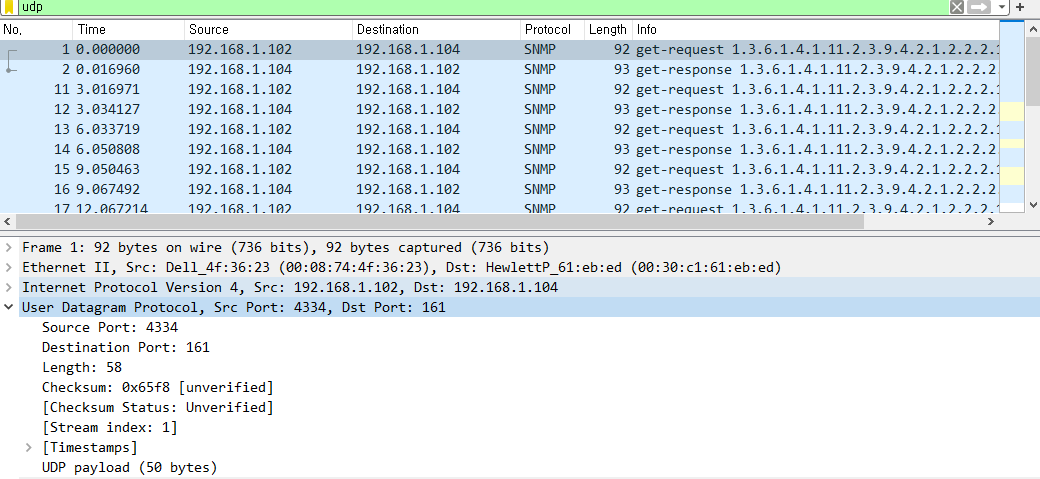
\includegraphics[width=.85\textwidth]{image/week02/2-1-1.png}
    		\caption{\footnotesize Problem 2-1's screenshot : }
    		\vspace{-10pt}
        \end{figure}
    %%%%%%%%%%%%%%%%%%%%%%%%%%%%%%%%%%%%%%%%%%%%%%%%% Problem 2-2
        \item By consulting the displayed information in Wireshark’s this packet packet content field for ,determine the length (in bytes) of each of the UDP header fields.\\[0.2mm]
        \soln
    %     \vspace{-4mm}  
    %     \begin{figure}[!h]\centering
    %     \hspace{15mm}  
    % 		\includegraphics[width=.85\textwidth]{image/week02/ }
    % 		\caption{\footnotesize Problem 2-2's screenshot : }
    % 		\vspace{-10pt}
    %     \end{figure}
    %%%%%%%%%%%%%%%%%%%%%%%%%%%%%%%%%%%%%%%%%%%%%%%%% Problem 2-3
        \item The value in the Length field is the length of what? this answer\\[0.2mm]
        \soln
    %     \vspace{-4mm}  
    %     \begin{figure}[!h]\centering
    %     \hspace{15mm}  
    % 		\includegraphics[width=.85\textwidth]{image/week02/ }
    % 		\caption{\footnotesize Problem 2-3's screenshot : }
    % 		\vspace{-10pt}
    %     \end{figure}
% \newpage
    %%%%%%%%%%%%%%%%%%%%%%%%%%%%%%%%%%%%%%%%%%%%%%%%% Problem 2-4
        \item What is the maximum number of bytes that c\\[0.2mm]
        \soln
    %     \vspace{-4mm}  
    %     \begin{figure}[!h]\centering
    %     \hspace{15mm}  
    % 		\includegraphics[width=.85\textwidth]{image/week02/ }
    % 		\caption{\footnotesize Problem 2-4's screenshot : }
    % 		\vspace{-10pt}
    %     \end{figure}
    %%%%%%%%%%%%%%%%%%%%%%%%%%%%%%%%%%%%%%%%%%%%%%%%% Problem 2-5
        \item What is the largest possible source port number?\\[0.2mm]
        \soln
    % \vspace{-4mm}  
    %     \begin{figure}[!h]\centering
    %     \hspace{15mm}  
    % 		\includegraphics[width=.85\textwidth]{image/week02/ }
    % 		\caption{\footnotesize Problem 2-5's screenshot : }
    % 		\vspace{-10pt}
    %     \end{figure}
    %%%%%%%%%%%%%%%%%%%%%%%%%%%%%%%%%%%%%%%%%%%%%%%%% Problem 2-6
        \item What is the protocol number for UDP? 
        Give your answer in both hex decimal notation. 
        To answer this question, you’ll need to loo adecimal and k into the field of the IP datagram containing this UDP segment.\\[0.2mm]
        \soln
    %     \vspace{-4mm}  
    %     \begin{figure}[!h]\centering
    %     \hspace{15mm}  
    % 		\includegraphics[width=.85\textwidth]{image/week02/ }
    % 		\caption{\footnotesize Problem 2-4's screenshot : }
    % 		\vspace{-10pt}
    %     \end{figure}
    \end{enumerate}
\newpage